\documentclass{article}
\usepackage{amssymb}

\usepackage{neurips_2026}
\usepackage{amssymb}

\usepackage[T1]{fontenc}
\usepackage[utf8]{inputenc}
\usepackage{microtype}
\usepackage{graphicx}
\usepackage{booktabs}
\usepackage{array}
\usepackage{amsmath}
\usepackage{enumitem}
\usepackage{xcolor}
\usepackage{hyperref}
\usepackage{float}
\usepackage{subcaption}
\usepackage{multirow}
\usepackage{nicefrac}

\newcommand{\pless}{P-less}
\newcommand{\best}[1]{\textbf{#1}}
\newcommand{\Qfour}{Q\textsubscript{4}}

\title{Long-Context Generation Is a Sampling Problem}

\author{
  Anonymous Author(s)
}

\begin{document}
\maketitle


\begin{abstract}
Long-form generation in open-weight language models collapses into repetition well before the context limit. We ask how much of that collapse the sampler controls. We rerun the full study from scratch in bf16 on ten instruction-tuned models from 1B to 120B parameters, adding natural-length continuation, non-fiction, a temperature-by-hyperparameter map, and long-horizon agentic coding on SWE-bench Verified. Two findings hold across every model. First, at the temperatures most systems ship, no truncation rule prevents collapse: forced to 16K tokens at $T{=}1$, top-$p$, min-$p$, P-less, Top-H and top-$n\sigma$ all end in a terminal loop in more than 95\% of generations, and a judge cannot separate them. Second, the sampler decides what happens once the temperature is raised to escape that loop, and a single measurable property predicts the outcome: how the realized candidate set responds to temperature. Rules whose candidate set grows with $T$ (top-$p$, top-$k$, Top-H) escape loops by admitting the noise tail and degrade into word salad, while top-$n\sigma$, whose candidate set is provably temperature invariant, keeps its local quality at $T{=}2$. We also correct the top-$n\sigma$ rule as stated in prior versions of this work and show that the commonly grouped ``full-distribution-aware'' samplers do not share a mechanism. Long-context generation is a sampling problem in a precise sense: sampling cannot rescue a model that wants to loop, but it determines whether the model survives the flattened distributions that long, high-temperature and agentic generation produce.
\end{abstract}

%% ====================================================================
\section{Introduction}
%% ====================================================================

Open-weight language models now accept and nominally generate very long sequences~\citep{dubey2024llama3,yang2024qwen2}. In practice the back half of a long sample frequently dissolves into repeated phrases, vocabulary narrowing, and loops~\citep{holtzman2020curious,welleck2020neural,fu2021theoretical}. The usual explanations point at model capacity and training data, and the usual fixes are retraining or long-output fine-tuning~\citep{bai2025longwriter}.

A competing explanation blames the sampler. Truncation rules such as top-$p$~\citep{holtzman2020curious} and top-$k$~\citep{fan2018hierarchical} were designed and validated on short outputs, and a family of newer rules, min-$p$~\citep{nguyen2024minp}, top-$n\sigma$~\citep{tang2024topnsigma}, Top-H~\citep{baghaei2025toph} and P-less~\citep{tan2025pless}, claims to adapt the candidate set to the shape of each step's distribution. If the sampler were the bottleneck, a better rule should hold long generations together without any training.

We test this claim directly, and we report what we find even where it cuts against the claim. Every experiment in this paper is a fresh run in bf16 with a single instrumented implementation of all samplers, verified against each method's reference code, which logs the realized candidate set at every decoding step.

\paragraph{Contributions.}
\begin{enumerate}[leftmargin=*,nosep]
\item \textbf{A negative result at deployment temperature.} Under forced 16K-token generation at $T{=}1$, every truncation rule we test ends in a terminal loop in more than 95\% of generations across ten models, and an LLM judge cannot separate them (Section~\ref{sec:r1}). Sampler choice does not prevent late-context collapse.
\item \textbf{The property that matters.} The sampler instead decides what happens when the temperature is raised to escape loops. We measure the realized candidate set and show that its response to temperature predicts the outcome: temperature-growing rules trade loops for word salad, while temperature-invariant top-$n\sigma$ keeps its local quality (Section~\ref{sec:mechanism}).
\item \textbf{Agentic and natural-length generation.} We extend the study to natural-length continuation, non-fiction, and long-horizon agentic coding on SWE-bench Verified, where the same property separates rules that keep an agent working at elevated temperature from rules that break it (Sections~\ref{sec:natural}--\ref{sec:agentic}).
\item \textbf{Corrections.} We correct the top-$n\sigma$ rule as stated in an earlier version of this work (Equation~\ref{eq:nsigma}) and show that the ``full-distribution-aware'' grouping does not correspond to a shared mechanism.
\end{enumerate}

%% ====================================================================
\section{Background and Related Work}
\label{sec:related}
%% ====================================================================

\paragraph{Truncation samplers.}
Temperature scaling divides logits by $T$ before the softmax~\citep{ackley1985learning}. Top-$k$ keeps the $k$ most probable tokens~\citep{fan2018hierarchical}. Top-$p$ keeps the smallest set whose cumulative probability exceeds $p$~\citep{holtzman2020curious}. Min-$p$ removes tokens below a fraction $p$ of the top probability~\citep{nguyen2024minp}. Locally typical sampling~\citep{meister2023locally}, $\eta$-sampling~\citep{hewitt2022truncation}, Mirostat~\citep{basu2021mirostat} and XTC~\citep{weidmann2024xtc} adapt the candidate set in other ways. Top-$n\sigma$~\citep{tang2024topnsigma}, Top-H~\citep{baghaei2025toph} and P-less~\citep{tan2025pless} condition the candidate set on statistics of the whole distribution and have been grouped as ``full-distribution-aware''. Section~\ref{sec:method} states each rule precisely.

\paragraph{Text degeneration and repetition.}
Neural text generation is prone to repetition during extended generation~\citep{holtzman2020curious,welleck2020neural,fu2021theoretical}. Repetition penalties~\citep{keskar2019ctrl}, diversity objectives~\citep{li2016diversity}, the DRY penalty~\citep{weidmann2024dry} and contrastive search~\citep{su2022contrastive,su2023contrastive} target the same symptom. We study the base truncation rule.

\paragraph{Long-context evaluation.}
Long-context capability is usually measured through retrieval and comprehension~\citep{bai2024longbench,hsieh2024ruler,shaham2023zeroscrolls}, while LongWriter~\citep{bai2025longwriter} probes length-following. LLM-as-judge evaluation~\citep{zheng2023judging,li2024generative} makes it practical to score long outputs window by window.

%% ====================================================================
\section{Samplers and the Temperature Response of the Candidate Set}
\label{sec:method}
%% ====================================================================

Let $\mathbf{z}\in\mathbb{R}^{|V|}$ be the logits at one step, $p=\mathrm{softmax}(\mathbf{z}/T)$ the tempered distribution, and $\mathcal{C}\subseteq V$ the candidate set from which the next token is sampled after renormalization. Following the order used by HuggingFace, vLLM and SGLang, every rule is applied to the tempered distribution.

\paragraph{P-less.}
P-less~\citep{tan2025pless} keeps tokens whose probability is at least the collision probability of the distribution:
\begin{equation}
L[p] = \sum_{v \in V} p(v)^2,
\qquad
\mathcal{C}_{\text{p-less}} = \{v \in V : p(v) \ge L[p]\}.
\label{eq:pless}
\end{equation}

\paragraph{Top-$n\sigma$.}
Top-$n\sigma$~\citep{tang2024topnsigma} keeps every token within $n$ standard deviations of the maximum logit:
\begin{equation}
\mathcal{C}_{\text{n-sigma}} = \{v \in V : z_v \ge \max_{u} z_u - n \cdot \sigma(\mathbf{z})\}.
\label{eq:nsigma}
\end{equation}
An earlier version of this paper stated the threshold as $\mu + n\sigma$. That rule is not top-$n\sigma$, and on Llama-3.1-8B it retains tens of thousands of tokens rather than a handful. All results here use Equation~\ref{eq:nsigma}.

\paragraph{Top-H.}
Top-H~\citep{baghaei2025toph} admits tokens in descending probability until the entropy of the renormalized set reaches a fraction $\alpha$ of $H(p)$. We use $\alpha{=}0.4$.

\paragraph{Temperature response.}
The property we will show to matter is how $\mathcal{C}$ changes with $T$. Dividing $\mathbf{z}$ by $T$ scales $\max_u z_u$ and $\sigma(\mathbf{z})$ equally, so the top-$n\sigma$ set is identical at every temperature~\citep{tang2024topnsigma}, and temperature only reshapes the probabilities inside it. Top-$k$ is also fixed by construction. Every other rule here thresholds on the tempered distribution itself, so its candidate set grows as $T$ flattens $p$: slowly for min-$p$ and P-less, whose thresholds are tied to the head of the distribution, and quickly for top-$p$ and Top-H, whose thresholds are tied to cumulative mass and entropy. Top-H therefore behaves like top-$p$ under temperature, not like top-$n\sigma$, even though both read a global statistic. We measure this response directly in Section~\ref{sec:mechanism}.

%% ====================================================================
\section{Experimental Setup}
\label{sec:setup}
%% ====================================================================

\paragraph{Models.}
The replication uses the ten models of the original study, updated to current checkpoints where the original was superseded: Llama-3.2-1B, Qwen2.5-1.5B, Qwen2.5-3B, Mistral-7B-v0.3, Llama-3.1-8B, Mistral-Nemo-12B, Qwen2.5-14B, Qwen2.5-32B, Llama-3.3-70B (all instruction-tuned)~\citep{dubey2024llama3,yang2024qwen2,jiang2023mistral}, and gpt-oss-120b. Extension studies add Qwen3.5, Gemma-4 and Qwen3 models where noted. All runs use unquantized bf16 weights on NVIDIA H200 GPUs (one RTX 5090 for the Qwen3-4B and Qwen3-8B sweeps).

\paragraph{Implementation.}
All samplers are implemented as one vLLM logits processor. Native vLLM sampling is disabled (temperature 1, top-$p$ 1, top-$k$ 0), so the processor is the only truncation and temperature rule. Each rule is checked row by row against its authors' reference implementation. Per decoding step the processor logs the entropy, the top probability, the candidate-set size, and the rank of the sampled token.

\paragraph{Protocols.}
\emph{Forced length} disables the end-of-sequence token until a fixed length (16K tokens). \emph{Natural length} allows the model to stop and continues it with a ``Continue.'' turn up to a 16K-token budget. Fiction prompts cover eight genres, and non-fiction prompts cover API references, design documents, code walkthroughs, test plans, protocol specifications and postmortems. Temperatures are $T\in\{1.0,1.5,2.0\}$ unless noted. Every wave was pre-registered, with its grid and primary outcome fixed before any output was read.

\paragraph{Outcomes.}
A generation has a \emph{terminal loop} if, from some 1K-token window onward, at least 80\% of the remaining windows have 32-gram repetition at least 0.5. An LLM judge (gpt-oss-120b) scores 1.5K-token windows at fixed depths for fluency, coherence, non-repetition, interest and overall quality on a 1--10 scale, and scores the whole output globally. We call a generation \emph{healthy} if it has no terminal loop and every judged window has coherence at least 6. Lexical diversity metrics are reported only as diagnostics, because word salad scores perfectly on them.

%% ====================================================================
\section{Results}
\label{sec:results}
%% ====================================================================

\subsection{At deployment temperature, no sampler prevents collapse}
\label{sec:r1}
% R1 table and text go here once all ten models are judged.

\subsection{The temperature response of the candidate set}
\label{sec:mechanism}
% cr_pool table goes here.

\subsection{Natural-length continuation and non-fiction}
\label{sec:natural}
% R2 / R4.

\subsection{Agentic coding}
\label{sec:agentic}
% R3 SWE-bench Verified, R6 LiveCodeBench.

%% ====================================================================
\bibliography{refs}
\bibliographystyle{plainnat}


%% ====================================================================
\newpage
\appendix

\section{Limitations}
\label{sec:limitations}

\paragraph{Model scale range.}
The study covers ten open-weight models from 1B to 120B parameters. Closed frontier models (e.g., the GPT-4 and Claude families) cannot be tested under our protocol because their sampler implementations are not user-controllable and their decoders are not exposed to the logit processor. Our results predict but do not measure their behavior at the scales we cannot reach.

\paragraph{Domain restriction.}
All experiments use creative fiction prompts. We chose fiction because late-context collapse is clearly visible in long narratives, but other domains (technical writing, multi-turn dialogue, code generation, agentic chains) may exhibit different failure modes or interact differently with the sampler. We expect the qualitative ordering to transfer because the underlying mechanism (the global-summary feedback loop) is domain-independent, but we have not directly verified this.

\paragraph{LLM-as-judge biases.}
The 21-metric judge protocol with GPT-4o~\citep{zheng2023judging} introduces known biases (length, style preference, position effects). We do not run a human evaluation, so every quality judgment in the paper rests on automatic metrics and LLM judges.

\paragraph{Inference setup.}
Models up to 32B run with 4-bit quantization on a single RTX 5090. The 70B and 120B runs use FP8 quantization on a 4xH100 cluster. Quantization can interact with sampling at very high temperature, where logit precision matters most. We have not tested fp16 baselines for the larger models.

\paragraph{Diagnostic scope.}
The selected-token rank is a useful one-dimensional diagnostic but cannot capture every form of distributional pathology. Long-form coherence failures that do not reduce to per-step distribution sharpening (e.g., factual drift, mid-story tone shifts) are not directly measured by the rank trajectory.

\paragraph{Implementation efficiency.}
Our \pless{} implementation is an unfused custom logit processor in SGLang. Throughput overhead is modest in our setup but could matter in latency-sensitive deployments. A fused implementation would close the gap, but we do not include one.


\section{Large 32K Campaign: 8B to 32B}
\label{app:large32k}

The 8B--32B campaign (four models, nine sampler configurations, eight genres, three seeds, 864 generations at 32K) confirms the small-scale finding that adaptive sampling holds final-quartile diversity near the ceiling while standard truncation collapses. \pless{} achieves the lowest repetition rate of any setting in the campaign and shows its strongest relative advantage on the largest model (Qwen2.5-32B), foreshadowing the frontier-scale picture in Section~\ref{sec:scale_campaign}. Mistral-Nemo is an instructive ceiling case where all samplers perform well at 32K. Figure~\ref{fig:hero-full} visualizes the cross-model collapse pattern.

\begin{table}[h]
\centering
\caption{\textbf{\pless{} achieves the lowest 10-gram repetition of any setting in the 8B--32B 32K campaign, with min-p at high temperature matching its diversity but missing on repetition.} Cross-model mean \Qfour{} metrics over three differentiating models (Llama-3.1-8B, Qwen2.5-14B, Qwen2.5-32B). Mistral-Nemo, which performs at ceiling regardless of sampler, is reported separately. Each cell averages 24 generations.}
\label{tab:large32k}
\small
\begin{tabular}{lcccc}
\toprule
Sampler & \Qfour{} d2 $\uparrow$ & \Qfour{} rep10 $\downarrow$ & \Qfour{} TTR $\uparrow$ \\
\midrule
\best{Min-p 0.1, $T{=}2.5$} & \best{0.935} & 0.042 & \best{0.706} \\
\pless{}, $T{=}1.9$ & 0.930 & \best{0.017} & 0.582 \\
\pless{}, $T{=}2.2$ & 0.903 & 0.046 & 0.571 \\
Min-p 0.1, $T{=}2.0$ & 0.643 & 0.081 & 0.406 \\
Temp-only, $T{=}1.0$ & 0.313 & 0.620 & 0.207 \\
Top-p 0.95, $T{=}1.0$ & 0.121 & 0.879 & 0.085 \\
Top-k 50, $T{=}1.0$ & 0.096 & 0.718 & 0.039 \\
Top-k 100, $T{=}1.0$ & 0.099 & 0.768 & 0.048 \\
Top-p 0.9, $T{=}1.0$ & 0.068 & 0.949 & 0.042 \\
\bottomrule
\end{tabular}
\end{table}

\begin{figure}[h]
\centering
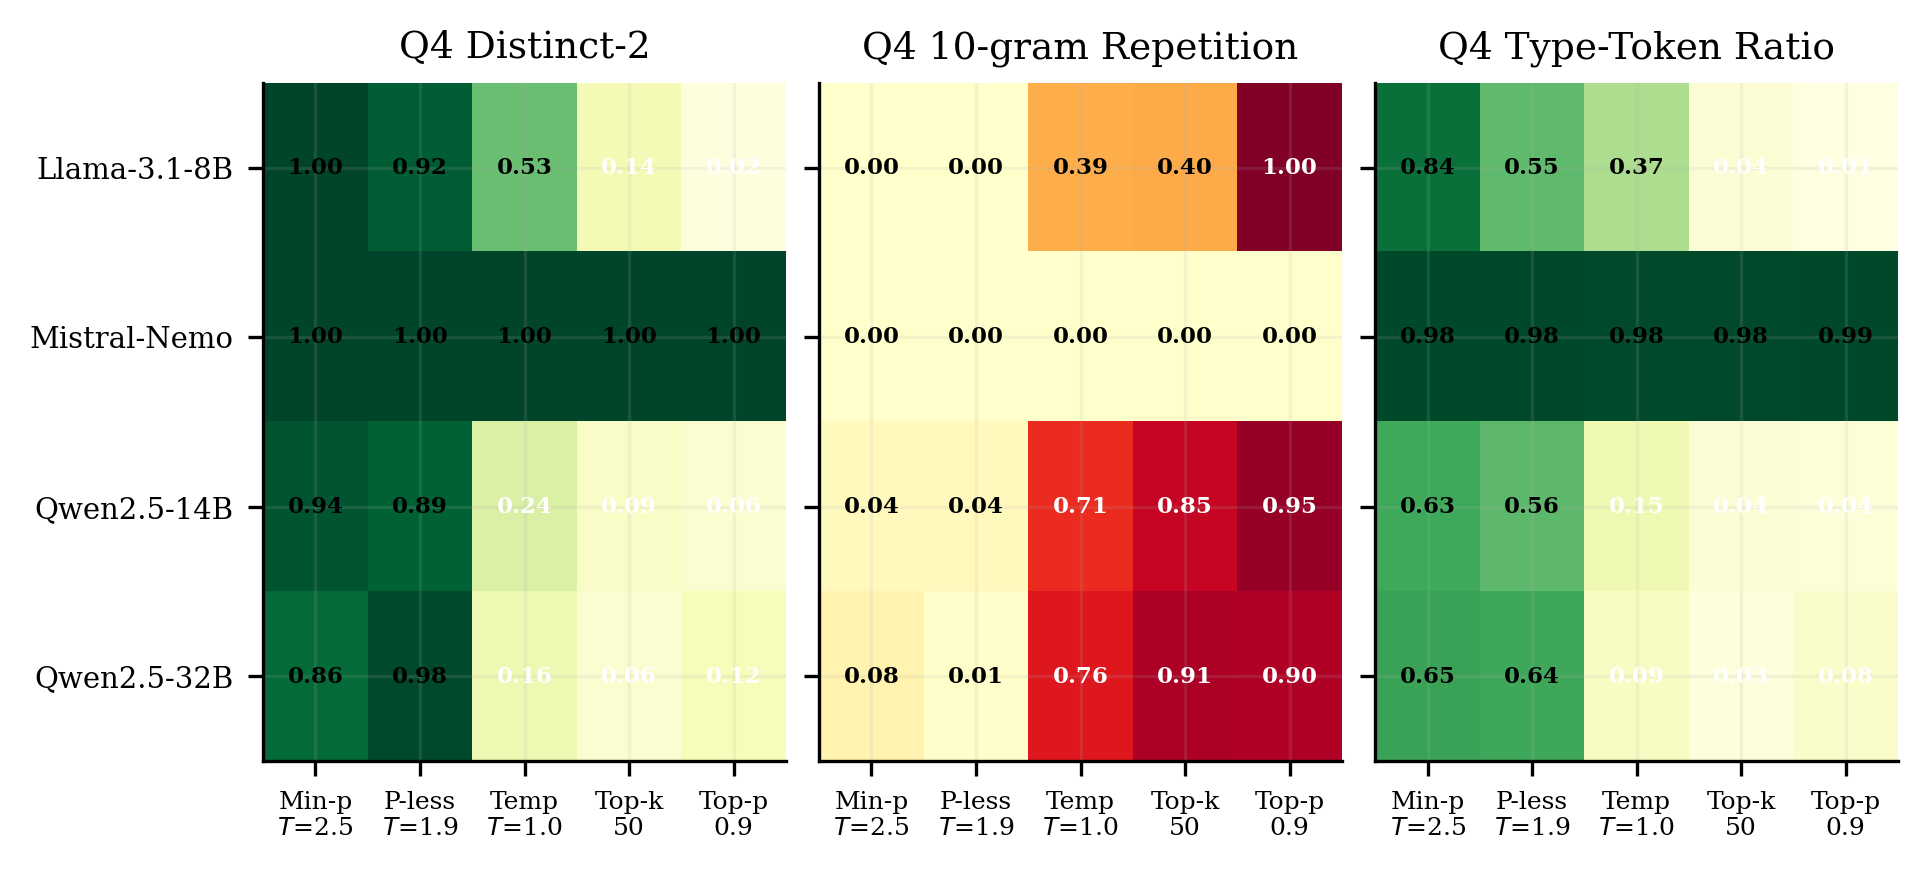
\includegraphics[width=\textwidth]{figures/fig_large_32k_campaign.png}
\caption{\textbf{Across four 8B--32B models at 32K, adaptive methods maintain high diversity and low repetition while standard truncation collapses. Mistral-Nemo is the ceiling case where all samplers perform well.} Final-quartile distinct-2 (top) and 10-gram repetition (bottom) per model.}
\label{fig:large32k}
\end{figure}


\section{Head-to-head \pless{} at 32K on Llama-3.1-8B}
\label{sec:32k_pless_app}

A head-to-head 32K study on Llama-3.1-8B anchors the temperature sweep used at frontier scale. \pless{} at $T{=}1.0$ achieves near-perfect distinct-2 with effectively zero 10-gram repetition, while top-k 50 and a weak min-p baseline collapse. The temperature sweep reveals $T{=}1.3$ as the optimal small-model operating point.

\begin{figure}[h]
\centering
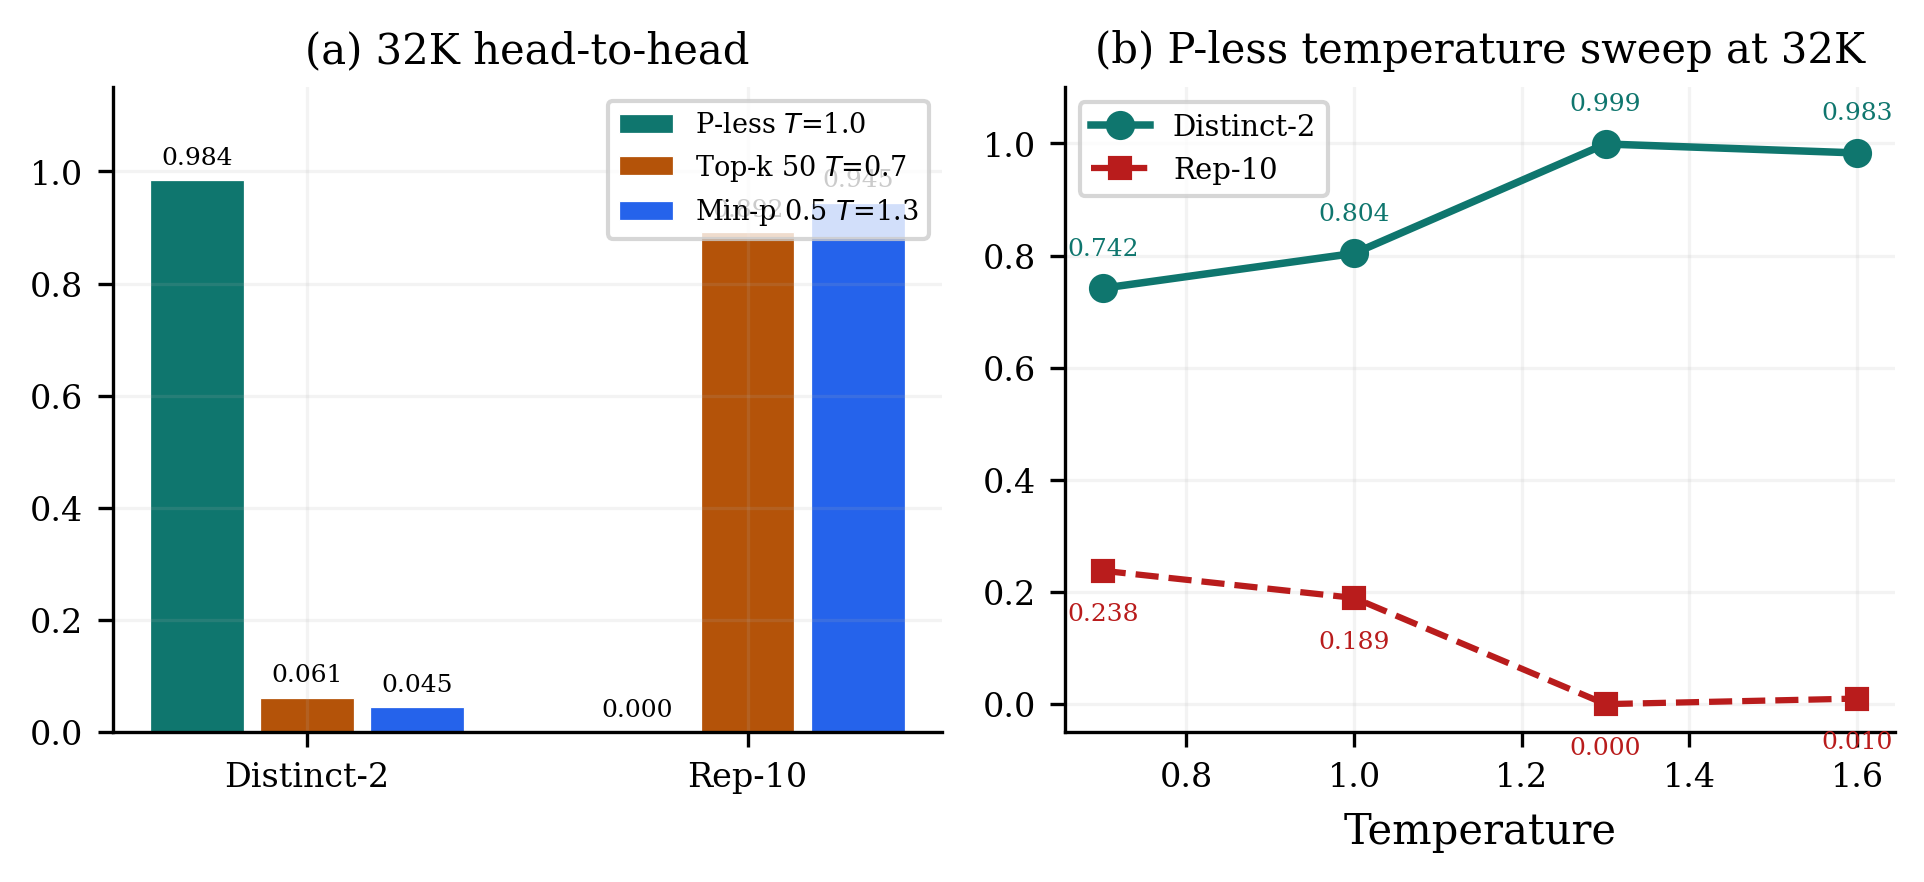
\includegraphics[width=0.75\textwidth]{figures/fig_32k_pless.png}
\caption{\textbf{\pless{} at $T{=}1.3$ is the small-model operating point: near-perfect distinct-2 and effectively zero 10-gram repetition.} \pless{} at 32K tokens on Llama-3.1-8B. (a) Head-to-head: \pless{} holds high distinct-2 and near-zero rep10 while top-k and a weak min-p baseline collapse. (b) Temperature sweep across $T{\in}\{1.0,1.3,1.6,1.9,2.2\}$.}
\label{fig:32k}
\end{figure}


\section{8K \pless{} Retune}
\label{app:retune}

Retuning the \pless{} temperature improves it substantially at small scale. The best small-scale operating point shifts from $T{=}1.3$ to $T{=}1.9$, where 10-gram repetition essentially vanishes and distinct-2 approaches the ceiling. Min-p still edges \pless{} on TTR at this scale, but the gap closes and reverses at frontier scale (Section~\ref{sec:scale_campaign}).


\section{Hero Figure: Late-Context Collapse at Scale}
\label{app:hero}

Figure~\ref{fig:hero-full} provides an expanded view of the final-quartile collapse phenomenon across all three differentiating models in the 32K campaign.

\begin{figure}[h]
\centering
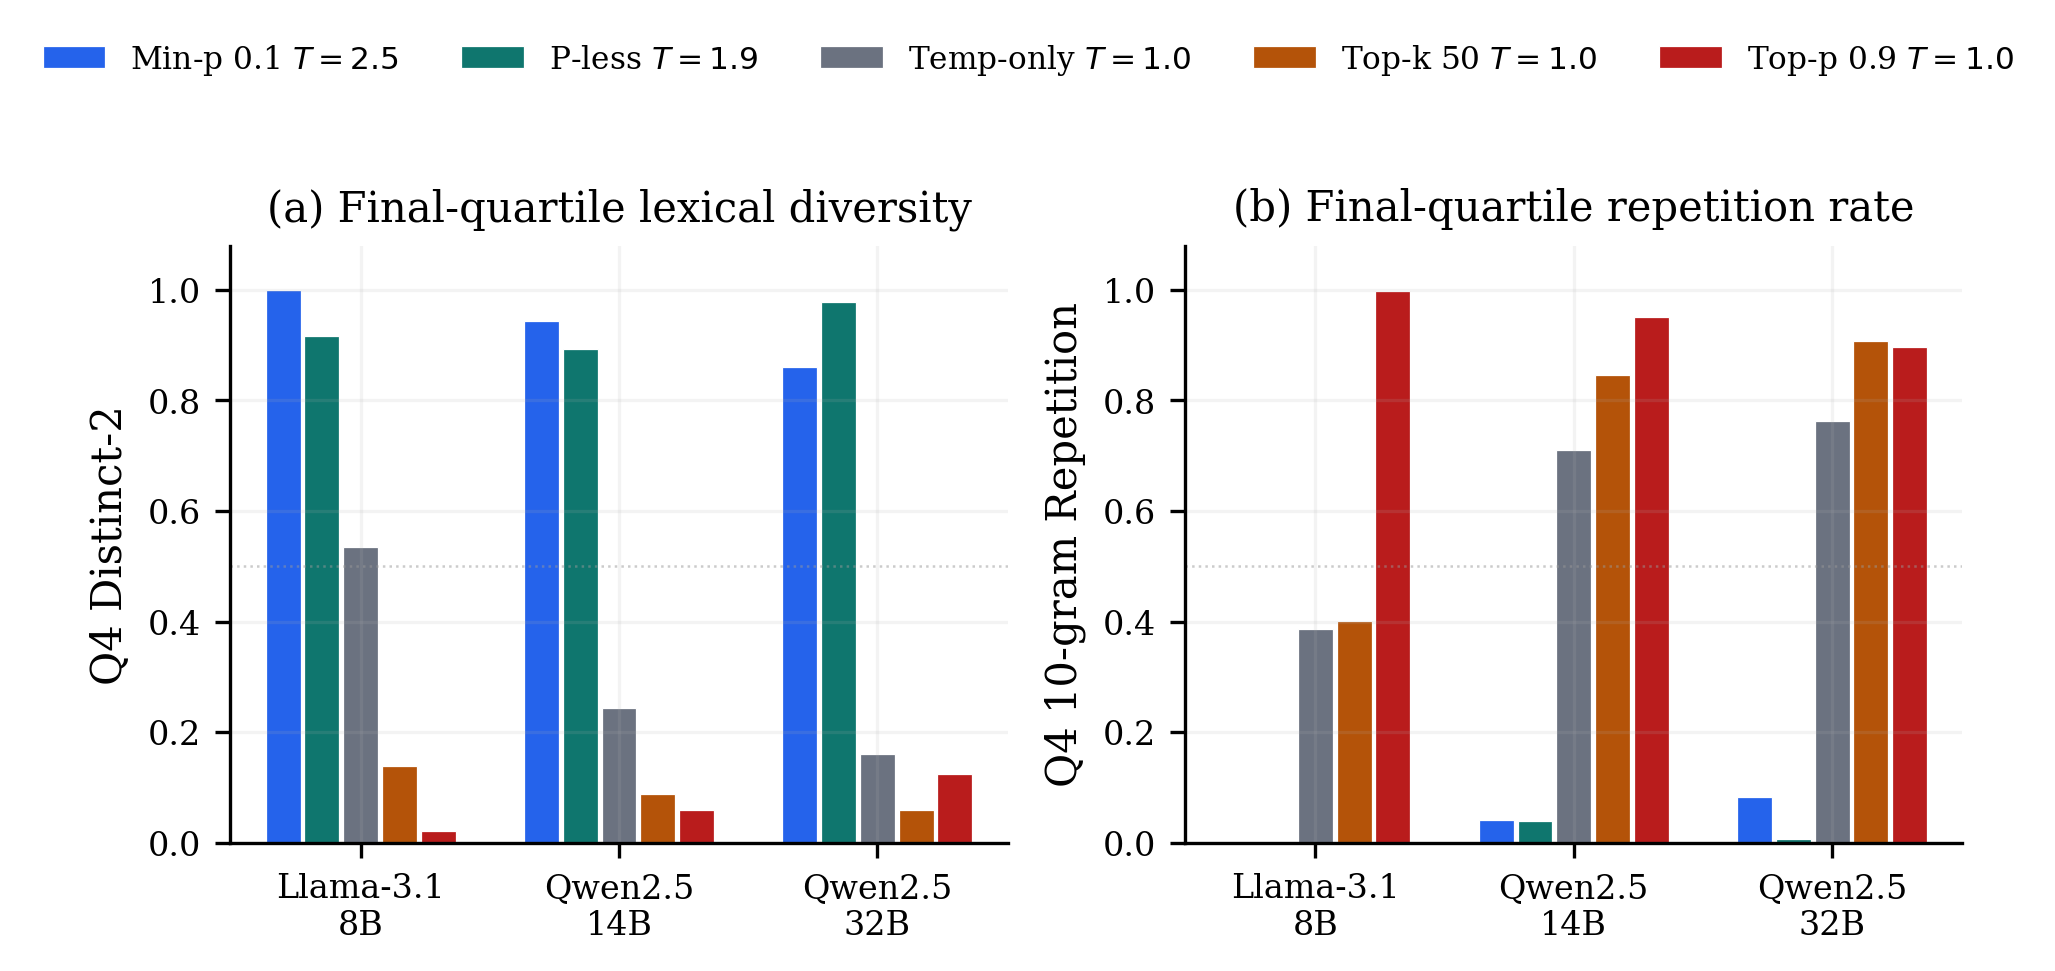
\includegraphics[width=\textwidth]{figures/fig_hero_degeneration.png}
\caption{\textbf{The advantage of adaptive sampling widens as model size grows, peaking on Qwen2.5-32B where standard truncation collapses to near-zero diversity.} Final-quartile metrics at 32K across 8B--32B models.}
\label{fig:hero-full}
\end{figure}


\section{21-Metric Judge Heatmap}
\label{app:judge_heatmap}

Figure~\ref{fig:judge-heatmap-app} shows the full 21-metric LLM-as-judge breakdown corresponding to Table~\ref{tab:judge-main}. The full-distribution-aware family (\pless{}, Top-H, top-$n\sigma$) leads on every metric family that captures long-range behavior, including long-range coherence, mid- and end-of-manuscript quality, stability, and overall quality. The metrics where standard truncation comes closest to the adaptive samplers are the short-window ones (grammar and beginning quality), which is consistent with the picture that long-context degeneration is the failure mode that distinguishes the families.

\begin{figure}[h]
\centering
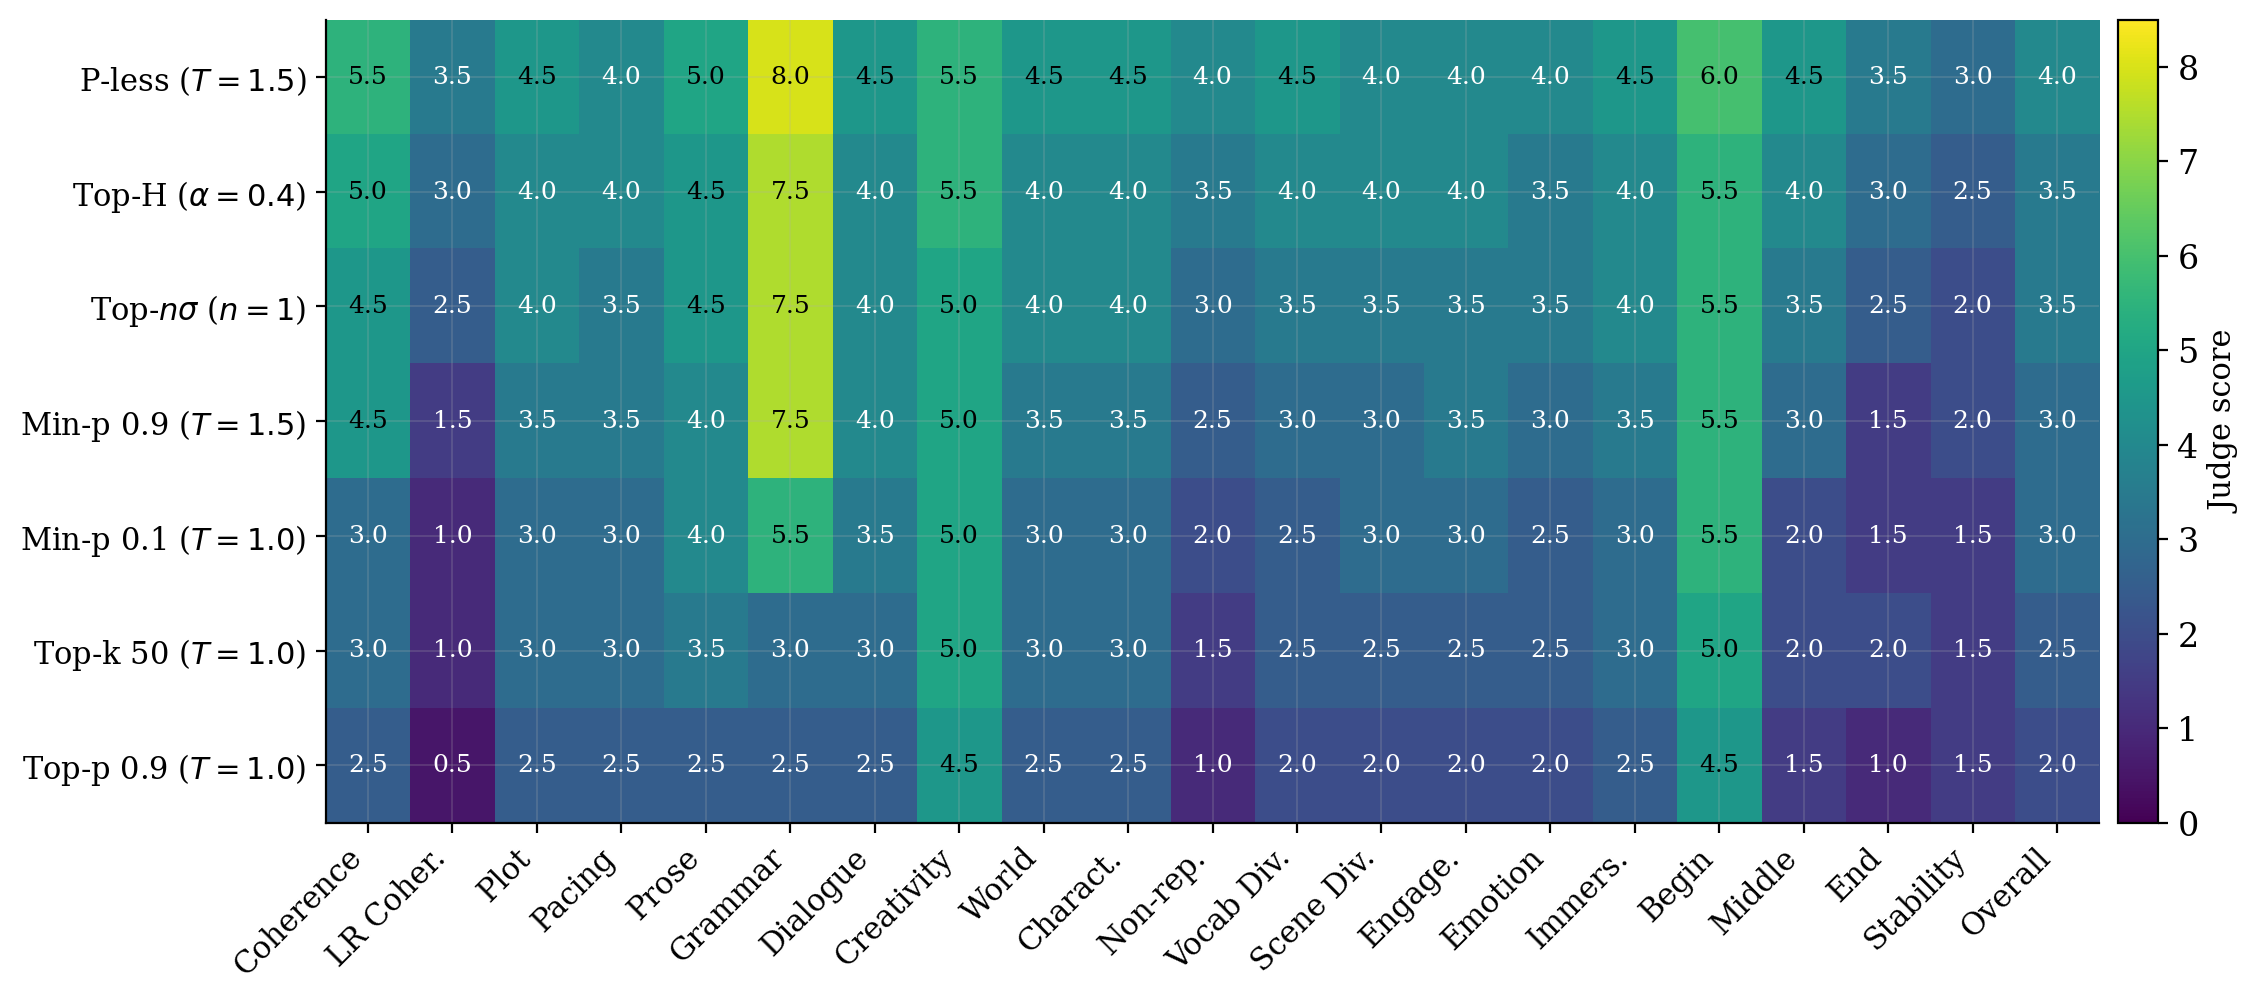
\includegraphics[width=0.85\textwidth]{figures/fig_judge_21metric.png}
\caption{\textbf{Full 21-metric heatmap supporting Table~\ref{tab:judge-main}.} The full-distribution-aware family leads on every metric that captures long-range behavior. Standard truncation closes the gap only on the short-window metrics (grammar, beginning quality).}
\label{fig:judge-heatmap-app}
\end{figure}


\section{$Q_1$ versus $Q_4$ Selected-Token Rank}
\label{app:q1q4}

The $Q_1$-versus-$Q_4$ aggregation accompanying Figure~\ref{fig:mstr_trajectory} is shown in Figure~\ref{fig:q1q4-app}. All samplers begin in the healthy 2.5--5 band. By $Q_4$, only the full-distribution-aware family stays there. Min-p drops below 2.0, and top-k and top-p land on the argmax floor near 1.0.

\begin{figure}[h]
\centering
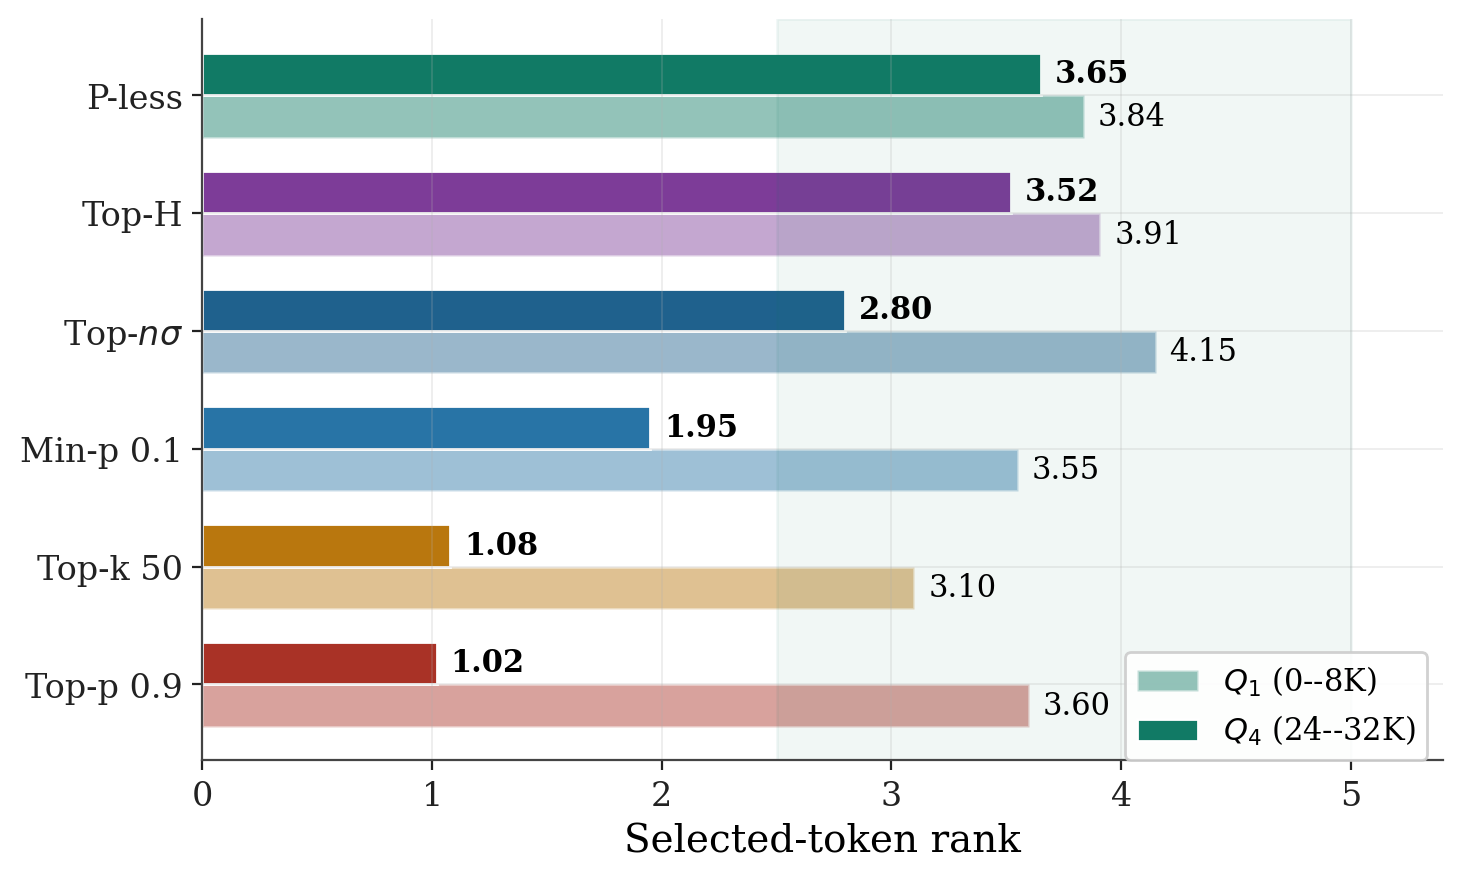
\includegraphics[width=0.7\textwidth]{figures/fig_q1q4_rank.png}
\caption{\textbf{All samplers begin in the healthy band, but only the full-distribution-aware family ends $Q_4$ there.} $Q_1$ versus $Q_4$ selected-token rank on Llama-3-70B at 32K. The shaded band marks the healthy 2.5--5 region. The dotted line at 1.0 is the argmax floor.}
\label{fig:q1q4-app}
\end{figure}


% NeurIPS Paper Checklist

\section*{NeurIPS Paper Checklist}

\begin{enumerate}

\item {\bf Claims}
    \item[] Question: Do the main claims made in the abstract and introduction accurately reflect the paper's contributions and scope?
    \item[] Answer: \answerYes{}
    \item[] Justification: The abstract states three claims (full-distribution-aware samplers dominate judged quality at frontier scale, min-p sits in a middle tier, and the gap widens with model scale) and each is supported by specific numbers from the experimental record. The three numbered contributions in the introduction map directly to the results sections.

\item {\bf Limitations}
    \item[] Question: Does the paper discuss the limitations of the work performed by the authors?
    \item[] Answer: \answerYes{}
    \item[] Justification: Section~\ref{sec:limitations} discusses model scale range (1B--120B open-weight only, no closed frontier models), domain restriction to creative fiction, LLM-as-judge biases, the small multi-model judged subset, the quantization-only inference setup, the one-dimensional nature of the selected-token rank diagnostic, and the unfused \pless{} implementation.

\item {\bf Theory Assumptions and Proofs}
    \item[] Question: For each theoretical result, does the paper provide the full set of assumptions and a complete (correct) proof?
    \item[] Answer: \answerNA{}
    \item[] Justification: This paper is empirical and does not contain theoretical results or proofs.

\item {\bf Experimental Result Reproducibility}
    \item[] Question: Does the paper fully disclose all the information needed to reproduce the main experimental results of the paper to the extent that it affects the main claims and/or conclusions of the paper?
    \item[] Answer: \answerYes{}
    \item[] Justification: Section~\ref{sec:setup} specifies the exact models, prompt genres, output lengths, sampler configurations, evaluation metrics, and infrastructure. Section~\ref{sec:method} describes the \pless{} algorithm. All sampler parameter values are reported in the tables.

\item {\bf Open access to data and code}
    \item[] Question: Does the paper provide open access to the data and code, with sufficient instructions to faithfully reproduce the main experimental results?
    \item[] Answer: \answerYes{Code and data will be released to the public upon acceptance.}  \href{https://anonymous.4open.science/r/long_context-20AE/}{Code is available here}
    \item[] Justification: The experimental codebase and generated outputs will be released as a public repository upon acceptance.

\item {\bf Experimental Setting/Details}
    \item[] Question: Does the paper specify all the training and test details necessary to understand the results?
    \item[] Answer: \answerYes{}
    \item[] Justification: All models are used off-the-shelf with no fine-tuning. Models up to 32B are inferred with SGLang on a single RTX 5090 with 4-bit quantization. The 70B and 120B runs use FP8 quantization on a 4xH100 cluster. All sampler parameters, temperatures, output lengths, and evaluation metrics are specified in Section~\ref{sec:setup}.

\item {\bf Experiment Statistical Significance}
    \item[] Question: Does the paper report error bars suitably and correctly defined or other appropriate information about the statistical significance of the experiments?
    \item[] Answer: \answerYes{}
    \item[] Justification: We report means over multiple generations per cell (3--24 depending on the study) and note sample sizes throughout. The 16K cross-model transfer figure (Figure~\ref{fig:transfer}) reports error bars from the across-model spread. The 32K campaign averages 24 generations per cell. We discuss the small multi-model judged subset as a limitation.

\item {\bf Experiments Compute Resources}
    \item[] Question: For each experiment, does the paper provide sufficient information on the computer resources needed to reproduce the experiments?
    \item[] Answer: \answerYes{}
    \item[] Justification: Models up to 32B run on a single NVIDIA RTX 5090 (32 GB) with 4-bit quantized models served through SGLang. The 70B and 120B runs use FP8 quantization on a 4xH100 cluster. The total compute is on the order of a few hundred GPU-hours.

\item {\bf Code Of Ethics}
    \item[] Question: Does the research conducted in the paper conform, in every respect, with the NeurIPS Code of Ethics?
    \item[] Answer: \answerYes{}
    \item[] Justification: The research studies open-weight language models on creative fiction generation. No personally identifying information is collected.

\item {\bf Broader Impacts}
    \item[] Question: Does the paper discuss both potential positive societal impacts and negative societal impacts of the work?
    \item[] Answer: \answerYes{}
    \item[] Justification: Improved long-context sampling lets open-weight models produce coherent long-form text without retraining, which lowers the cost of high-quality generation for low-resource users and reduces the energy cost of post-training fixes. The same improvement applies to misuse cases (longer fluent disinformation, longer phishing). The underlying models already enable both, and our contribution is a sampler-level change that does not unlock new capabilities beyond what the base models support.

\item {\bf Safeguards}
    \item[] Question: Does the paper describe safeguards that have been put in place for responsible disclosure of data with personal or offensive content?
    \item[] Answer: \answerYes{}
    \item[] Justification: The generated outputs are creative fiction from non-adversarial standard prompts. We screened the prompt set to exclude topics that would induce graphic or unsafe content from the underlying models. The released artifact will be the sampler implementation and aggregate evaluation scripts, not the raw generations.

\item {\bf Licenses for existing assets}
    \item[] Question: Are the creators or original owners of assets used in the paper properly credited and are the license and terms of use explicitly mentioned and properly respected?
    \item[] Answer: \answerYes{}
    \item[] Justification: All models used are open-weight and properly cited. SGLang is cited. No proprietary datasets are used.

\item {\bf New Assets}
    \item[] Question: Are new assets introduced in the paper well documented and is the documentation provided alongside the assets?
    \item[] Answer: \answerYes{The \pless{} sampler implementation and evaluation scripts will be released with documentation.}
    \item[] Justification: The \pless{} algorithm is described in Section~\ref{sec:method}. Code release is planned upon acceptance.

\item {\bf Crowdsourcing and Research with Human Subjects}
    \item[] Question: For crowdsourcing experiments and research with human subjects, does the paper include the full text of instructions given to participants and screenshots, if applicable, as well as details about compensation?
    \item[] Answer: \answerNA{}
    \item[] Justification: The paper does not involve crowdsourcing or research with human subjects.

\item {\bf Institutional Review Board (IRB) Approvals or Equivalent for Research with Human Subjects}
    \item[] Question: Does the paper describe potential risks incurred by study participants, whether such risks were disclosed to the subjects, and whether Institutional Review Board (IRB) approvals were obtained?
    \item[] Answer: \answerNA{}
    \item[] Justification: The paper does not involve research with human subjects.

\item {\bf Declaration of LLM usage}
    \item[] Question: Does the paper describe the usage of LLMs if it is an important, original, or non-standard component of the core methods in this research?
    \item[] Answer: \answerYes{}
    \item[] Justification: GPT-4o is used as the LLM judge in our 21-metric evaluation protocol (Section~\ref{sec:setup}). The paper itself studies sampling algorithms for open-weight LLMs across ten models (Llama, Qwen, Mistral, GPT-OSS), all of which are documented in Section~\ref{sec:setup}. LLMs were not used in the writing of the paper beyond standard editing assistance, which does not affect the core methods or claims.

\end{enumerate}


\end{document}
